% Appendix A

\chapter{Características adicionales del hardware} % Main appendix title

\label{AppendixA} % For referencing this appendix elsewhere, use \ref{AppendixA}

Este apéndice presenta las especificaciones técnicas detalladas de los componentes de hardware utilizados en el desarrollo del instrumento. Se incluyen las características eléctricas del sensor SPS30, las especificaciones de alimentación de la placa STM32F429ZI y su distribución de puertos. Adicionalmente, se detallan las características técnicas de los módulos complementarios: microSD para almacenamiento, ESP8266 para comunicación inalámbrica y DHT22 para medición de variables ambientales. Por último, se especifica la instrumentación utilizada durante el desarrollo y validación del sistema.

%\section{Características adicionales sensor \MPF} % Main appendix title

%\label{AppendixB} % For referencing this appendix elsewhere, use \ref{AppendixA}

\begin{table}[tph]
	\small
	\centering
	\caption{Características eléctricas del SPS30 \cite{Sensirion2023}.}
	\label{tab:electrical_characteristics}
	%\begin{table}
%\centering
%\caption{Características eléctricas SPS30 \cite{Sensirion2023}}
%\label{tab:electrical_characteristics}
\begin{tabular}{p{4.4cm}p{3.cm}lll}
	\toprule
	\textbf{Parámetro} & \textbf{Condiciones} & \textbf{Min} & \textbf{Typ} & \textbf{Max} \\ 
	\midrule
	Voltaje de alimentación & & \SI{4.5}{\volt} & \SI{5.0}{\volt} & \SI{5.5}{\volt} \\
	Corriente de suministro & Modo dormido & - & \SI{38}{\micro\ampere} & \SI{50}{\micro\ampere} \\ 
	Corriente de suministro & Modo inactivo & \SI{300}{\milli\ampere} & \SI{330}{\milli\ampere} & \SI{360}{\milli\ampere} \\ 
	Corriente de suministro & Modo medición & \SI{45}{\milli\ampere} & \SI{55}{\milli\ampere} & \SI{65}{\milli\ampere} \\ 
	Corriente de suministro & Primeros \SI{200}{\milli\second} (inicio ventilador) & - & - & \SI{80}{\milli\ampere} \\ 
	Voltaje de entrada nivel alto & & - & \SI{2.31}{\volt} & \SI{5.5}{\volt} \\ 
	Voltaje de entrada nivel bajo & & \SI{0}{\volt} & \SI{2.9}{\volt} & \SI{0.99}{\volt} \\ 
	Voltaje de salida nivel alto & & - & \SI{3.3}{\volt} & \SI{3.37}{\volt} \\ 
	Voltaje de salida nivel bajo & & \SI{0}{\volt} & \SI{0}{\volt} & \SI{0.4}{\volt} \\ 
	\bottomrule
\end{tabular}
%\end{table}
\end{table}

%\section{Características adicionales de la placa SMT32F429ZI}

\begin{table}[h]
	\small
	\centering
	\caption{Fuentes de alimentación externas del STM32F429ZI. %\citep{waveshare_nucleo_f429zi}.
	}
	\label{tab:external_power_sources}
%!TEX root = ../memoria.tex
%\begin{table}[h]
%	\centering
%	\caption{Fuentes de alimentación externas}
%	\label{tab:external_power_sources}
\begin{tabular}{@{}p{2cm}p{2.3cm}p{2cm}p{3cm}@{}}
	\toprule
	Nombre de la entrada & Pines del conector & Rango de voltaje & Límite de corriente máxima \\ 
	\midrule
	\multirow{3}{*}{VIN} & CN8 pin 15 & \multirow{3}{*}{\SIrange{7}{12}{\volt}} & \SI{800}{\milli\ampere} (\SI{7}{\volt})\\ 
	& CN11 pin 24 & & \SI{450}{\milli\ampere} (\SIrange{7}{9}{\volt})\\ 
	& & & \SI{250}{\milli\ampere} (\SIrange{9}{12}{\volt}) \\ 
	E5V & CN11 pin 6 & \SIrange{4.75}{5.25}{\volt} & \SI{500}{\milli\ampere} \\ 
	+3,3 V & CN8 pin 7, CN11 pin 16 & \SIrange{3.0}{3.6}{\volt} & - \\ 
	\bottomrule
\end{tabular}
%\end{table}



\end{table}

\begin{figure}
	\centering
	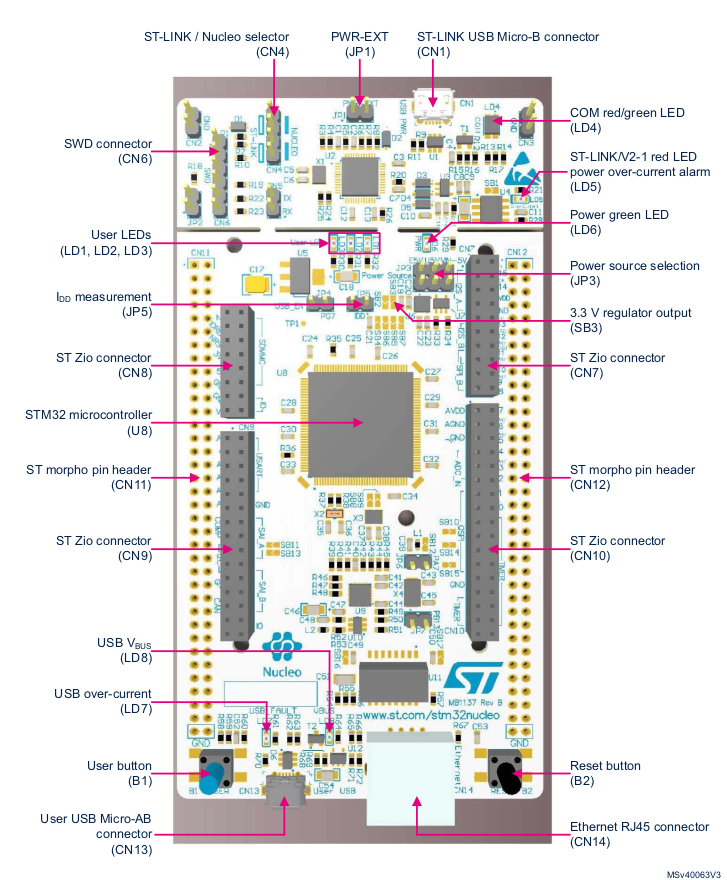
\includegraphics[width=1\linewidth]{Figures/placanucleoF429ZI}
	\caption{Placa de desarrollo utilizada para el  trabajo, con sus principales puertos. %\citep{waveshare_nucleo_f429zi}.
	}
	\label{fig:placanucleof429zi}
\end{figure}

%\section{Módulo de comunicación DHT22}

\begin{table}[h!]
	\centering
	
	\caption{Especificaciones técnicas del sensor DHT22. %\citep{Aosong2023}.
	}
	\small
		\begin{tabular}{ll}
	\toprule
	\textbf{Parámetro} & \textbf{Valor} \\
	\midrule
	Tensión de operación & \SI{3.3}{\volt} - \SI{5.5}{\volt} \\
	Corriente típica & \SI{2.5}{\milli\ampere} \\
	Rango de humedad & \SIrange{0}{10}{\RH} \\
	Precisión humedad & \SI{\pm2}{\RH} \\
	Rango temperatura & \SI{-40}{\celsius} - \SI{80}{\celsius} \\
	Precisión temperatura & $\pm$\SI{0.5}{\celsius} \\
	Tasa de muestreo & \SI{0.5}{\hertz} \\
	Tiempo de respuesta humedad & \SI{2}{\second} \\
	Tiempo de respuesta temperatura & \SI{10}{\second} \\
	\bottomrule
\end{tabular}

	\label{tab:dht22_specs}
\end{table}






%\section{Módulo microSD}
\begin{table}[h!]
	\centering
	\caption{Especificaciones del módulo microSD. %\cite{SDCard2020, FatFs2022}.
	}
	\small
	\begin{tabular}{ll}
		\toprule
		\textbf{Parámetro} & \textbf{Especificación} \\
		\midrule
		Protocolo & SPI \\
		Velocidad máxima & \SI{42}{\mega\hertz} \\
		Tensión de operación & \SIrange{3.3}{5}{\volt} \\
		Consumo en escritura & \SI{200}{\milli\ampere} \\
		Sistema de archivos & FAT32 \\
		Capacidad máxima & \SI{32}{\giga\byte} \\
		\bottomrule
	\end{tabular}
	\label{tab:microsd_specs}
\end{table}

%\section{Módulo de comunicación ESP8266}

\begin{table}[htbp]
	\centering
	\small
	\caption{Características principales del módulo ESP8266. %\cite{Espressif2020}.
	}
	\label{table:esp8266_specs}
	%	\caption{Características principales del módulo ESP8266}
%	\label{table:esp8266_specs}
	\begin{tabular}{ll}
		\toprule
		\textbf{Característica} & \textbf{Especificación} \\
		\midrule
		Procesador & CPU RISC de 32 bits Tensilica L106 \\
		Frecuencia de operación & \SI{80}{\mega\hertz} - \SI{160}{\mega\hertz} \\
		Memoria RAM & \SI{160}{\kilo\byte} \\
		Memoria Flash & \SI{512}{\kilo\byte} - \SI{4}{\mega\byte} \\
		Tensión de alimentación & \SIrange{3.0}{3.6}{\volt} \\
		Consumo en modo activo & \SI{80}{\milli\ampere} \\
		Consumo en modo sleep & \SI{20}{\micro\ampere} \\
		Protocolos Wi-Fi & 802.11 b/g/n \\
		Seguridad Wi-Fi & WPA/WPA2 \\
		Rango de frecuencia Wi-Fi & \SI{2.4}{\giga\hertz} \\
		Potencia de transmisión & \SI{19.5}{\dBm} \\
		Interfaces & UART/SDIO/SPI/I2C/I2S/GPIO \\
		Rango de temperatura & \SIrange{-40}{125}{\celsius} \\
		Certificaciones & FCC/CE/TELEC/SRRC \\
		\bottomrule
	\end{tabular}
\end{table}



\begin{table}[htbp]
	\caption{Instrumentación y herramientas de prueba.}
	\label{tab:pruebas}
	\small
	\centering
	\begin{tabular}{lll}
		\hline
		\textbf{Instrumento} & \textbf{Modelo} & \textbf{Especificaciones} \\
		\hline
		Analizador lógico & - & \SI{24}{\mega\hertz}, 8 canales \\
		Osciloscopio & FNIRSI1014D & \SI{100}{\mega\hertz} \\
		Multímetro & TMT460012 & Digital \\
		Fuente de poder & Jesverty SPS-3005 & \SIrange{0}{30}{\volt}, \SI{5}{\ampere} \\
		Medidor MP & Grimm & Analizador óptico \\
		Framework pruebas & Ceedling & Testing unitario en C \\
		\hline
	\end{tabular}
\end{table}


\begin{table}[!hbp]
	\centering
	\small
	\caption{Especificaciones de los instrumentos empleados en el banco de pruebas.}
	\label{tab:pruebas2}
	\begin{tabular}{p{0.20\linewidth}p{0.18\linewidth}p{0.52\linewidth}}
		\toprule
		\textbf{Instrumento} & \textbf{Modelo} & \textbf{Función en la validación del sistema} \\
		\bottomrule
		Analizador lógico & USBee AX Pro (\SI{24}{\mega\hertz}, 8 canales) & Verificación de protocolos de comunicación (\IIC, SPI, UART) y análisis de sincronización entre componentes del sistema \\
		
		Osciloscopio digital & FNIRSI-1014D (\SI{100}{\mega\hertz}, \SI{1}{\giga\hertz} tasa de muestreo) & Caracterización de señales analógicas y digitales, medición de ruido, análisis de transitorios e integridad de señal \\
		
		Multímetro digital & TMT460012 (precisión: \SI{\pm0.5}{\percent}) & Medición de parámetros eléctricos (tensión, corriente, resistencia) y verificación de puntos de prueba \\
		
		Analizador de potencia USB & Aideepen UM34C & Monitorización en tiempo real de consumo energético (\SI{0}{\ampere}--\SI{3}{\ampere}, \SI{0}{\volt}--\SI{26}{\volt}) y eficiencia del sistema \\
		
		Fuente de alimentación & Jesverty SPS-3005 (\SIrange{0}{30}{\volt}, \SI{5}{\ampere}) & Suministro controlado y estabilizado de energía, simulación de condiciones de alimentación variables \\
		
		Monitor de referencia \MPF & Grimm 11-D & Validación metrológica de concentraciones de material particulado con precisión certificada (\SI{\pm2}{\percent}) \\
		
		Analizador por atenuación beta & Met One BAM-1022 & Sistema de referencia EPA-equivalente para calibración y verificación a largo plazo \\
		
		Software CAD electrónico & KiCad 6.0 & Verificación de reglas de diseño del PCB, análisis de integridad de señal y compatibilidad electromagnética \\
		
		Medidor LCR & FNIRSI LCR-P1 (\SIrange{100}{100000}{\hertz}) & Caracterización de componentes pasivos con precisión de \SI{0.3}{\percent} para validación de tolerancias \\
		
		Framework de pruebas & Ceedling 0.31.1 con Unity/CMock & Automatización de pruebas unitarias, generación de objetos simulados y cobertura de código para el firmware \\
		
		Terminal serial & Cutecom 0.51.0 & Monitorización de comunicaciones serie, verificación de protocolos y análisis de flujos de datos \\
		\bottomrule
	\end{tabular}
\end{table}



